\documentclass[10pt,a4paper]{article}
\usepackage{adjustbox}
\usepackage[utf8]{inputenc}
\usepackage[spanish, es-tabla]{babel}
\usepackage{listings}
\usepackage{pdfpages}
\usepackage{pythontex} 
\usepackage{listingsutf8}
\lstset{basicstyle=\footnotesize\ttfamily}
\lstset{language=Python, breaklines=true, frame=single, keywordstyle=\bfseries}
\lstset{numbers=left, numberstyle=\tiny, stepnumber=1, numbersep=3mm, tabsize=3}
\usepackage[dvipsnames,svgnames]{xcolor}
\usepackage{enumitem}
\usepackage{amsmath}
	\numberwithin{equation}{section}
	\numberwithin{figure}{section}
	\numberwithin{table}{section}
\usepackage{subfigure}
\usepackage{booktabs}
\usepackage[hang,bf,justification=centering]{caption}
\usepackage{amsfonts}
\usepackage{amssymb}
\usepackage{gensymb}
\usepackage{lscape}
\usepackage{gensymb}
\usepackage{hyperref}
\usepackage[normalem]{ulem}
\useunder{\uline}{\ul}{}
\usepackage{algorithm,algorithmic}

\usepackage{graphicx}
	\graphicspath
	{
		{Images/} 
	}
\usepackage{indentfirst}
\usepackage{geometry}
 	\geometry
 	{
		a4paper, 
		total	= {210mm,297mm},
		left	= 20mm,
		right	= 20mm,
		top		= 20mm,
		bottom	= 20mm,
	}
\usepackage{float}
\usepackage{fancyhdr}
\pagestyle{fancy}
\rhead{Dr. Rodriguez, Daniel -  Manchiunas, Valeria}
\lhead{75.12 - Análisis Numérico}
\lfoot{Moreno,Vicari}
\rfoot{Universidad de Buenos Aires}
\cfoot{\thepage}



\begin{document}

% ----------------------%
% 		CARATULA 		%
%-----------------------%

\title{TP 1 NUMÉRICO }    


\begin{titlepage}
%%%%%%%%%%%%%%%%%%%%%%%%%%%
%%%%%%%%%%%%%%%%%%%%%%%%%%%%%%%%%555
	\vspace*{30mm}

	\begin{center}
	    
\includegraphics[scale=1.2]{../Images/Logo_Fiuba2.png}\\
		\huge{\textsc{Universidad de Buenos Aires}}\\
		\huge{\textsc{Facultad de Ingeniería}}\\
		\vspace*{5mm}
		\large{Año 2021 - 1.\textsuperscript{er} cuatrimestre}
	\end{center}

	\vspace*{15mm}

	\begin{center}
		\huge{\underline{\textsc{ANÁLISIS Y NUMÉRICO (75.12 - 95.04)}}}\\
		\vspace*{5mm}
		\large{Curso 06 - Rodriguez - Machiunas}
	\end{center}

	\vspace*{5mm}

	\begin{large}
			
	\begin{tabbing}
		\hspace{15mm} \= \+	
		\textsc{TRABAJO PRÁCTICO DE MÁQUINA N.º 1}\\
		
         
		\textsc{Integrantes:}\\
	
%	\vspace*{10mm}
	
		\begin{tabular}{ l l l }
			
          
			
            
             86559 & Vicari, Dario Santiago		&  dvicari@fi.uba.ar\\
             88019 & Moreno, Jorge              &  jomoreno@fi.uba.ar\\
             

		\end{tabular}
	 
	\end{tabbing}
	
	\end{large}
	
	\hspace{15mm} \textsc{Fecha de entrega:} 12/06/2021  	\hspace{15mm} 
	
\end{titlepage}


\setcounter{page}{1}


\section{\underline{Enunciado}}

La altura de las mareas se puede modelar utilizando una sumatoria de componentes armónicas de acuerdo a la siguiente ecuación:

\begin{equation}\label{eq_1}
    \begin{split}
        altura = a_0 + \Big[\sum_{k=1}^{n} a_k  \cos(\omega_k t + \Phi_k)\Big] 
    \end{split}
\end{equation}\\

Siendo:
$a_0$: nivel medio de referencia\\
$n$: número de componentes armónicas consideradas\\
$\omega_k$: frecuencia angular de la componente armónica k-ésima\\
$\phi_k$: fase de la componente armónica k-ésima\\

Los parámetros de la ecuación \ref*{eq_1} se calculan a partir de la serie temporal de datos obtenida por mareógrafos en los años anteriores, conocida como marea astronómica. Por lo general los responsables de la toma de datos de los mareógrafos son organismos que dependen de los gobiernos.\\
Históricamente se realizaba una publicación llamada anuario de mareas y en ocasiones también se publicaban las últimas constantes armónicas obtenidas en los puertos principales.\\
Actualmente parte de la información es de acceso público a través de páginas web. Por ejemplo, en Argentina, el organismo responsable es el Servicio de Hidrografía Naval. \url{http://www.hidro.gov.ar}. Cada puerto tiene asociada una tabla de mareas y en ocasiones hay que realizar correcciones debido a la influencia de los factores meteorológicos.\\
\\
El primer objetivo de este TP es estimar las constantes armónicas de un puerto, del cual se dispone la altura de la marea en forma horaria, durante un año.\\
\\
Cada grupo elegirá una combinación de puerto/año diferente, de un conjunto suministrado por los docentes.[ Publique en el foro del TP 1 su puerto/año de esta primer parte, y verifique que no haya sido elegido por otro grupo]\\
\\
Para cumplir adecuadamente el objetivo propuesto se sugiere se realicen los siguientes pasos:
\begin{enumerate}
    \item 
    Determinen las frecuencias angulares más importantes $(\omega_1$,$\omega_2$,$\omega_3$,...$\omega_n)$. Para ello utilicen la transformada discreta de Fourier. Podrán utilizar la implementación de la transformada rápida de Fourier (fft) en Octave o Python. Deberán indicar que criterio utilizan para definir la cantidad de componentes armónicas ($n$). (En caso de consultar bibliografía adicional, recuerden tomar nota de los datos de la misma, para citarla en la bibliografía).
    \item
    Utilicen el método de mínimos cuadrados para obtener el nivel medio de referencia $(a_0)$ y la amplitud de cada componente armónica $(a_1,a_2,...,a_n)$ seleccionada previamente, como así también la fase. Indicar el ECM.
    \item
    Repitan el punto anterior pero utilizando una componente armónica menos y analicen el efecto de esta modificación.
    \item
    Repitan los puntos anteriores, pero esta vez utilizando solamente 
    \begin{enumerate}
        \item
        los datos de la primer semana de enero;
        \item
        los datos de la segunda semana de enero;
        \item
        los datos de enero y febrero;
        \item
        los datos de marzo y abril;
    \end{enumerate}
    Comparen (y relacionen, si les parece que es posible) los valores obtenidos en los componentes armónicos.
    \item
    Suponga ahora que se desea realizar predicciones diarias de las horas y alturas de las pleamares y bajamares utilizando únicamente una sola componente armónica de acuerdo a la siguiente ecuación:
    \begin{equation}\label{eq_2}
        \begin{split}
            altura = a_0 + a_1 cos(\omega_1 t + \phi_1)
        \end{split}
    \end{equation}
    Indiquen como se modifican los parámetros $(a_0,\omega_1,\phi_1)$ si solo se desea predecir las pleamares y bajamares en el mes de enero y en el mes de marzo
    (Pueden complementar el análisis empleando 2 o hasta 3 componentes armónicas, si les parece necesario; justifiquen su elección, en ese caso).
    \item
    Ahora vamos utilizar la ecuación \ref{eq_2} para predecir las mareas en los puertos de la costa Argentina.
    Los datos se obtendrán de la página:
    \url{http://www.hidro.gov.ar/oceanografia/Tmareas/Form_Tmareas.asp} seleccionelo de la lista de puertos patrones; y cada grupo elegirá un puerto diferente. [Publiquen en el foro del TP 1 su puerto para esta segunda parte, y verifique que no haya sido elegido por otro grupo].
    
    Tomen los datos completos de marzo, abril y los primeros 21 días de mayo de este año. (Observe que los datos no son equiespaciados). Se aconseja que procesen los datos horarios y luego copien todo a un archivo de texto, para cargarlo con facilidad en Octave o Python.
    Para poder utilizar el modelo lineal de cuadrados mínimos, primero hagan gráficos y estudien que valor de $\omega_1$ es adecuado utilizar -a partir de la inspección de los datos- y expliquen el criterio utilizado; luego por cuadrados mínimos lineales estime los parámetros $a_0$,$a_1$ y $\phi_1$.
    También pueden optar por emplear el modelo de cuadrados mínimos no lineal.
    Hallen el ECM.\\
    
    \item
    Utilicen el modelo obtenido en el punto anterior para predecir la hora de la primer pleamar de junio de la playa elegida. Expliquen la estrategia utilizada para la modelización.
    
\end{enumerate}


\section{\underline{Introducción}}

En este Trabajo Práctico, tenemos como objetivo utilizar el método de cuadrados mínimos para modelar la altura de las mareas en distintos puertos, en nuestro caso, el puerto de Maine, y el puerto de Mar del Plata.
Ambos puertos registran las alturas de la marea, pero la diferencia es que en el primer caso, esta se registra de forma horaria, y en el segundo caso se registra solo para las pleamares y bajamares.
Estos dos casos distintos nos harán utilizar distintas metodologías para hallar los modelos.

\section{\underline{Desarrollo}}

En el primer caso, el del puerto de Maine, procesamos el archivo .csv dado, y 

Partiendo de la ecuación \ref*{eq_1}, y aplicando la identidad trigonométrica $ \cos(\alpha+\beta) = \cos(\alpha)\cos(\beta) - \sin(\alpha)\sin(\beta) $:

\begin{equation}\label{eqn:eq_3}
    \begin{split}
        altura_n(t) &= a_0 + \sum_{k=1}^{n} a_k \cos(\omega_k t + \phi_k) \\
                  &= a_0 + \sum_{k=1}^{n} a_k  \cos(\omega_k t)\cos(\phi_k) -  \sin(\omega_k t)\sin(\phi_k)  \\
                  &= a_0 + \sum_{k=1}^{n} \underbrace{a_k \cos(\phi_k)}_{A_k} \cos(\omega_k t) + \underbrace{ - a_k \sin(\phi_k)}_{B_k} \sin(\omega_k t) \\
                  &= a_0 + \sum_{k=1}^{n} A_k \cos(\omega_k t)  + \sum_{k=1}^{n} B_k \sin(\omega_k t)
    \end{split}    
\end{equation}

Donde los coeficientes $A_k$ y $B_k$ quedan caracterizados de la siguiente manera:
\begin{equation}\label{eqn:eq_3_1}
    \begin{split}
        A_k &= a_k*\cos(\phi_k)
    \end{split}
\end{equation}
\begin{equation}\label{eqn:eq_3_2}
    \begin{split}
        B_k &= -a_k*\sin(\phi_k)
    \end{split}
\end{equation}

Los valores $a_k$ y $\phi_k$ son los coeficientes de la Transformada Rápida de Fourier (FFT), el valor $a_0$, que sería el valor medio, la altura media, se puede calcular
utilizando el método de cuadrados mínimos, como la constante que minimiza el error cuadrático Medio. Los coeficientes de fourier minimizan el Error Cuadrático Medio como se puede ver en \cite{ana2}, Capítulo 8.5, teorema 8.13.
Como vemos a continuación. Estos desarrollos  se tomaron de \cite{ana1} capítulo 4.2:

\begin{equation}\label{eq_4}
    \begin{split}
        EC = \parallel f(x) - \hat{f}(x) \parallel^2 = \sum_{k=1}^{n} \omega_k (f(x_k)-\hat{f}(x_k))^2
    \end{split}
\end{equation}
Error Cuadrático Medio

\begin{equation}\label{eq_4_2}
    \begin{split}
        ECM =  \frac{\sqrt{\parallel f(x) - \hat{f}(x) \parallel^2 = \sum_{k=1}^{n} \omega_k (f(x_k)-\hat{f}(x_k))^2}}{n}
    \end{split}
\end{equation}
Para determinar cuantos armónicos fueron necesarios para recrear una serie que minimice el ECM, ordenamos de mayor a menor los coeficientes de la FFT y obteniendo las posiciones dentro del vector resultado, luego se toman los mayores $n$ armónicos y se arma la serie.
Fuimos iterando y hallamos que a partir de pocos armónicos, relativos a la cantidad total, había un amesetamiento en la reduccion del ECM.

Fundamentalmente, el método de los cuadrados mínimos, se trata de hallar una función $\hat{f}(x)$ que minimice el error cuadrático $EC$, partiendo de un conjunto
 de $n \in \mathbb{N}$ de valores $(x_i,y_i)$, donde consideramos $f(x_i) = y_i$, luego:

\begin{equation}\label{eq_5}
    \begin{split}
        \hat{f}(x) &= \sum_{i=1}^{m} c_i \phi_i(x)  
    \end{split}
\end{equation}

Reemplazando \ref*{eq_5} en \ref*{eq_4} defino al Error Cuadrático como una funcion $g(\vec{c}), \vec{c} \in \mathbb{R}^n $ que dependa de las constantes $c_i$:

\begin{equation}\label{eq_6}
    \begin{split}
        g(c_1,\ldots,c_m) &= \sum_{k=1}^n \omega_k ( f(x_k) - \sum_{j=1}^m  c_j \phi_j(x_k))^2\\
    \end{split}
\end{equation}
Lo que buscamos entonces, es minimizar el Error Cuadrático en funcion de los $C_i$, para ello:

\begin{equation}\label{eq_7}
    \begin{split}
        \frac{\partial g }{\partial c_j} &= 0 \qquad 1 \leq j \leq n \\
        \frac{\partial g }{\partial c_j} &= \frac{\partial \big( \sum\limits_{i=1}^m ( f(x_i) - \sum\limits_{i=1}^n  c_i \phi_i)^2 \big) }{\partial c_j}  \\
        &= \sum_{k=1}^m 2\omega_k (f(x_k)) - \sum_{i=1}^n c_i \phi_i) (-\phi_j) = 0
    \end{split}
\end{equation}        
\begin{equation}\label{eq_8}
     \begin{split}
        \sum_{k=1}^m \omega_k f(x_k) \phi_j = \sum_{k=1}^m \sum_{i=1}^n c_i \omega_k \phi_i \phi_j
     \end{split}
\end{equation}

\begin{equation}\label{eq_9}
    \begin{split}
       \sum_{k=1}^m \omega_k f(x_k) \phi_j = \sum_{i=1}^n c_i ( \sum_{k=1}^m  \omega_k \phi_i \phi_j )
    \end{split}
\end{equation}
Debemos definir entonces el pseudo producto escalar entre dos funciones como:
\begin{equation}\label{eq_10}
    \begin{split}
        (f,g) = \sum_{k=1}^m \omega_k f(x_k) g(x_k)
    \end{split}
\end{equation}
Usando la definición \ref*{eq_10} en \ref*{eq_9} obtenemos:
\begin{equation}\label{eq_11}
    \begin{split}
        (f,\phi_j) = \sum_{i=1}^n c_i (\phi_i,\phi_j)
    \end{split}
\end{equation}
Con los datos de entrada de ejemplo, en los cuales contamos con un par ordenado de ${x_i,y_i}$, nos interesa aproximar $\hat{f}(x) = c \phi(x)$ donde $\phi(x) = 1)$. Entonces a partir de la ecuación \ref*{eq_11}
y tomando el valor $\omega_k = 1$:
\begin{equation}
    \begin{split}
        (f,\phi) = c(\phi,\phi) \Longrightarrow c &= \frac{(f,\phi)}{(\phi,\phi)} = \frac{\sum\limits_{k=1}^m f(x_k)}{\sum\limits_{k=1}^m 1 = m} \\
        c &= \frac{\sum\limits_{k=1}^m y_k}{m} = \bar{y}
    \end{split}
\end{equation}


El el último item, se presenta una serie de datos ${x_i,y_i}$ que no estan equiespaciados, dejando el análisis de los términos de fourier fuera de utilidad, aunque claro podríamos 
utilizar una interpolación y muestrar equidistantemente dicha interpolación, pero es un caso que podemos obviar si utilizamos diréctamente el método de cuadrados mínimos.
Para ello utilizamos la ecuación \ref*{eqn:eq_3} para un armónico:
\begin{equation}\label{eq_12}
    \begin{split}
        altura_1(t) &= a_0 + a_1 \cos(\omega_1 t) + b_1 \sin(\omega_1 t)
    \end{split}
\end{equation}
Reescribimos la ecuación en función de la definicion de \ref*{eq_5}:
\begin{equation}\label{eq_13}
    \begin{split}
        altura_1(t) &= c_1 * \phi_1(t) + c_2 \phi_2(t) + c_3 \phi_3(t)
    \end{split}
\end{equation}
Donde:
\begin{equation}\label{eq_14}
    \begin{split}
        \phi_1(t) &= 1 \\
        \phi_2(t) &= \cos(\omega_1 t)\\
        \phi_3(t) &= \sin(\omega_1 t)\\
    \end{split}
\end{equation}
Entonces debemos resolver el sistema usando las definiciones de las ecuaciones \ref*{eq_10} y \ref*{eq_11}
\begin{equation}\label{eq_15}
    \begin{bmatrix}
        (\phi_1,\phi_1) & (\phi_1,\phi_2) & (\phi_1,\phi_3)\\
        (\phi_2,\phi_1) & (\phi_2,\phi_2) & (\phi_2,\phi_3)\\
        (\phi_3,\phi_1) & (\phi_3,\phi_2) & (\phi_3,\phi_3)
    \end{bmatrix} * 
    \begin{bmatrix}
        c_1\\
        c_2\\
        c_3
    \end{bmatrix} =
    \begin{bmatrix}
        (f,\phi_1)\\
        (f,\phi_2)\\
        (f,\phi_3)
    \end{bmatrix}
\end{equation}

Esto resulta en un sistema lineal, que resolvemos utilizando python para obtener los valores de las constantes y utilizar el modelo deseado.

    
\section{\underline{Resultados}}

Hallamos la fft, y graficamos los armónicos para ver que podíamos observar:\\
\begin{minipage}{\textwidth}
\centering
    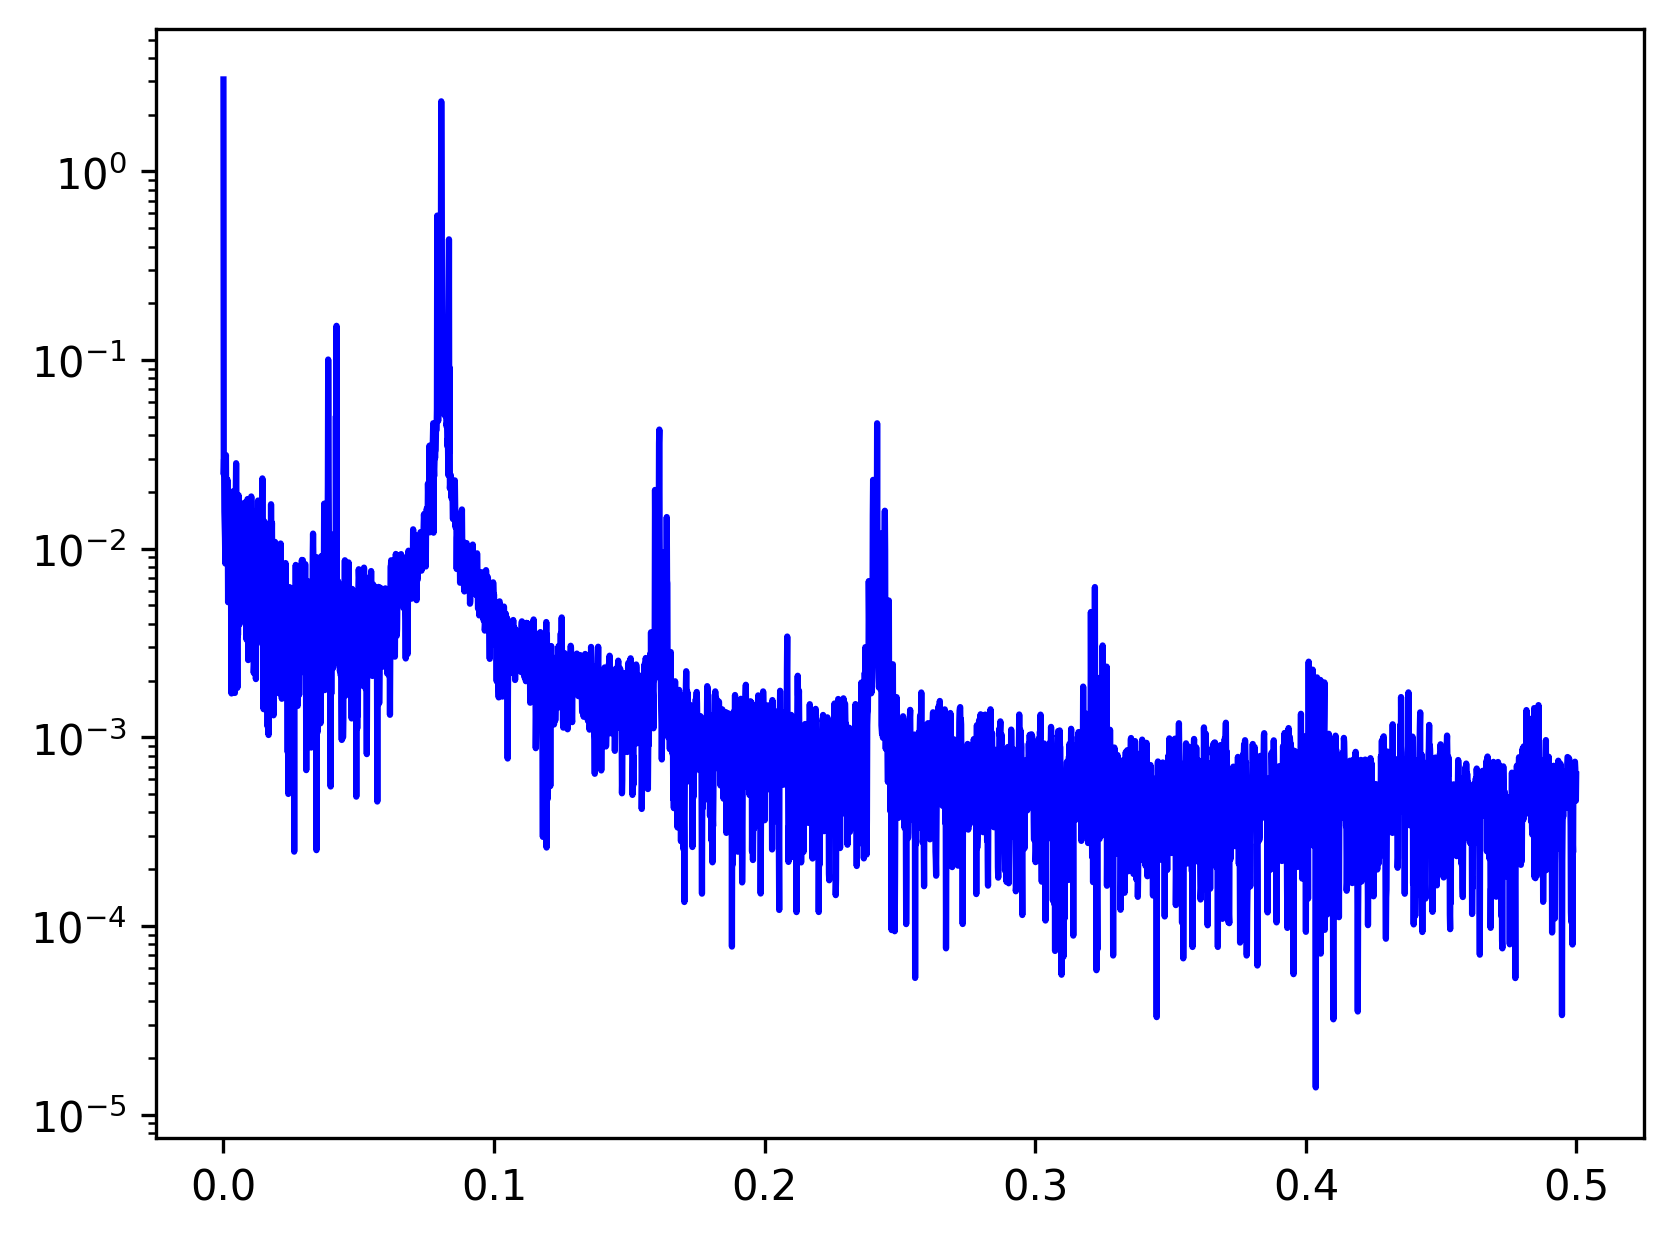
\includegraphics[scale=1]{ Images/ejercicio_a_fft_log.png}\\
 \captionof{figure}{Modulo de la amplitud de fourier para las alturas de las mareas}
 \label{fig:fig1}
\end{minipage}
Luego graficamos el Error Cuadratico Medio  Para decidir con cuantos armónicos trabajar con nuestros modelos:
\begin{minipage}{\textwidth}
    \centering
        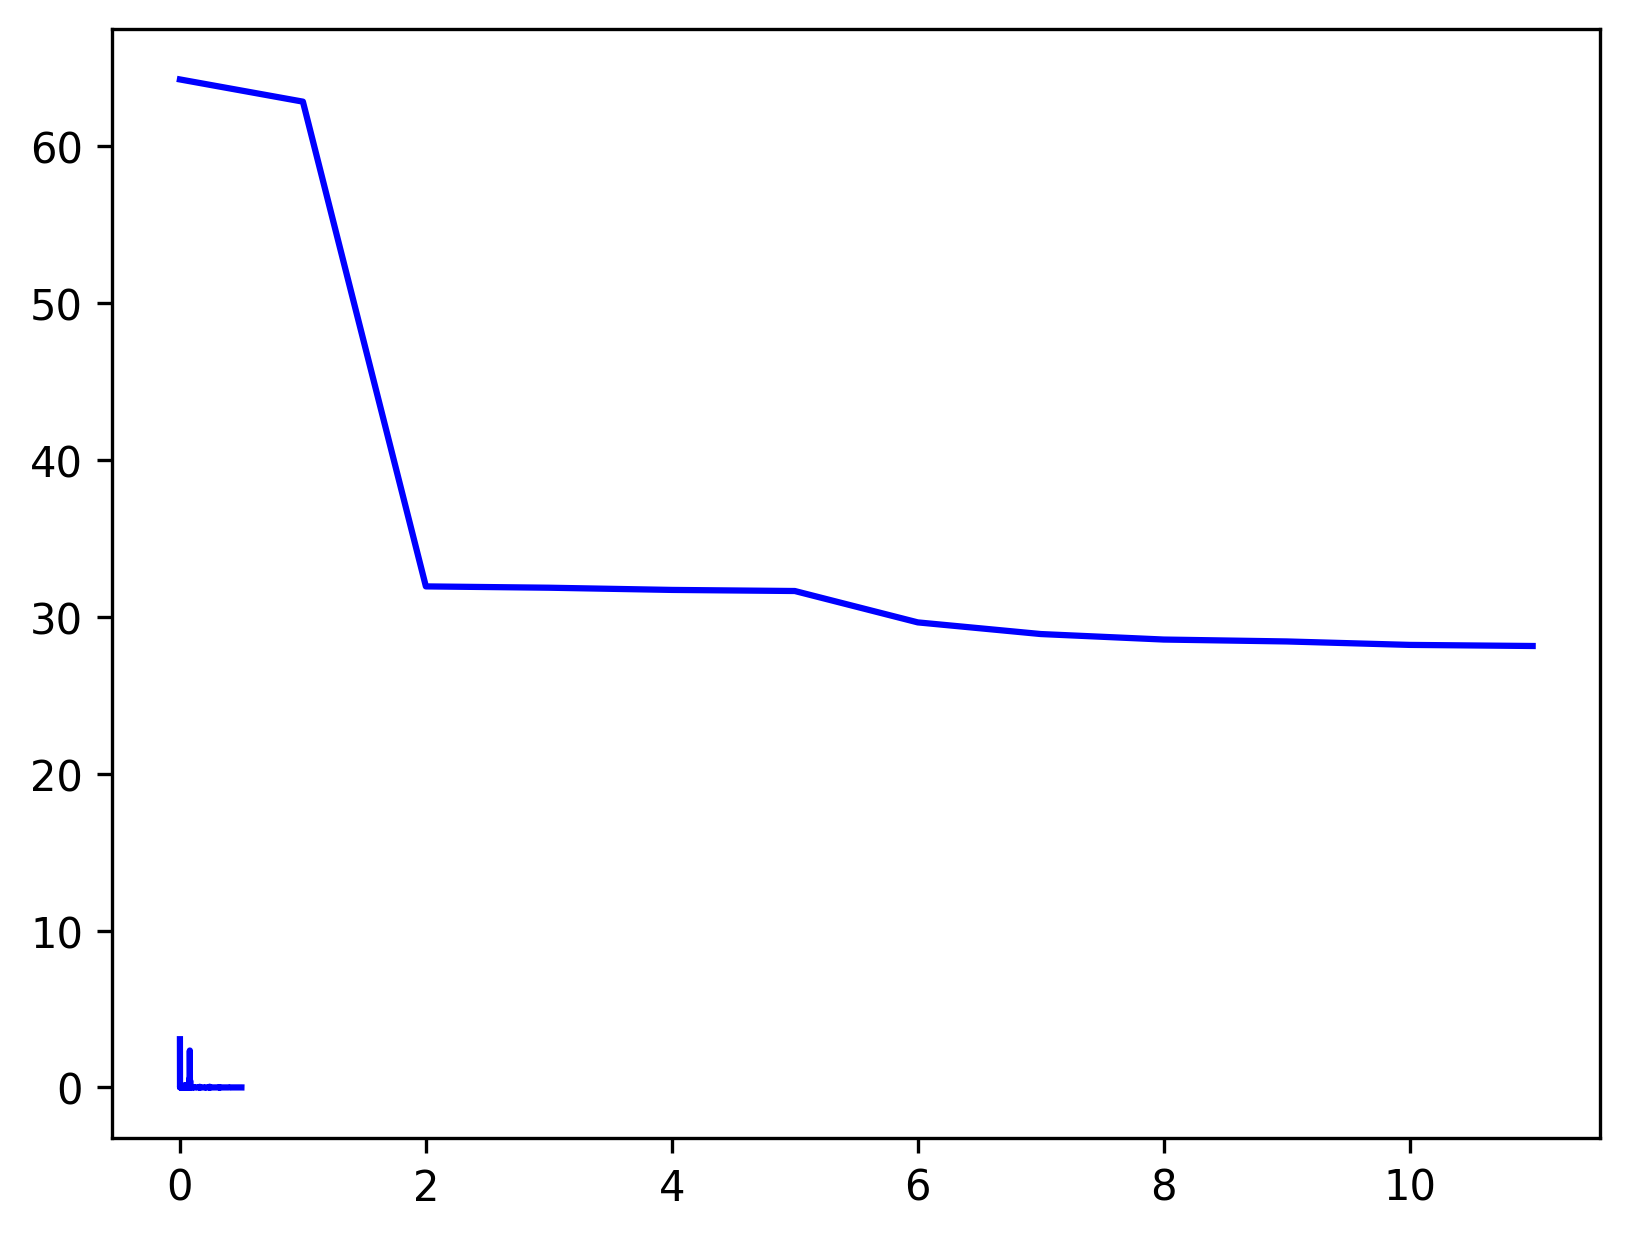
\includegraphics[scale=1]{ Images/ejercicio_a_ecm_x_12armonicos.png}\\
     \captionof{figure}{Error Cuadratico Medio en funcion de los armónicos usados}
     \label{fig:fig2}
\end{minipage}

Decidimos a partir de este resultado utilizar 4 muestras, con esto calculamos los ejercicios b,c y d donde obtuvimos los siguientes resultados y los tabulamos:

\begin{center}
    \begin{tabular}{||c|c|c|c||} 
    \hline
    Rango & Número de Armonicos & E.C.M. & Frecuencias \\ [0.5ex] 
    \hline\hline
    Todo & 4 & 0.9797659067456904 &  [0.         0.03869863 0.07899543 0.08047945] \\ 
    \hline
    Todo & 3 &  0.9823491454457174 & [0.         0.07899543 0.08047945] \\
    \hline
    Primer Semana de Enero & 4 & 1.2367958297155777 & [0.         0.08333333 0.08928571 0.0952381 ] \\
    \hline
    Primer Semana de Enero & 3 &  1.2659584466847664 & [0.         0.08333333 0.08928571 ] \\
    \hline
    Segunda Semana de Enero & 4 &  1.4869772458332933 & [0.         0.06547619 0.07142857 0.07738095]  \\
    \hline
    Segunda Semana de Enero & 3 & 1.500698778195625  &  [0.         0.06547619 0.07142857] \\
    \hline
    Enero y Febrero & 4  & 0.6826298627212011 & [0.         0.07904023 0.07974594 0.08045166] \\
    \hline
    Enero y Febrero & 3  & 0.6696914537749843 &  [0.         0.07904023 0.07974594 0.08045166]\\
    \hline
    Marzo y Abril & 4  & 0.6826298627212011 &[0.         0.07904023 0.07974594 0.08045166] \\
    \hline
    Marzo y Abril & 3  &  0.6696914537749843&[0.         0.07904023 0.07974594 0.08045166] \\
    \hline
   \end{tabular}
   \end{center}

   Para el siguiente ejercicio, obtuvimos los armonicos y calculamos:

\begin{verbatim}
    Valor Medio Enero (a_0):  3.1356599462365593 , Primer Armónico (a_1):  2.6293397521253157  Frecuencia Angular (w_1):  0.5067084925144828  Fase 1 (phi_1):  0.1522951793391947
    Valor Medio marzo (a_0):  3.033045698924731 , Primer Armónico (a_1):  2.5921290112734927  Frecuencia Angular (w_1):  0.5067084925144828  Fase 1 (phi_1):  0.21275576895293635 
\end{verbatim}

\begin{minipage}{\textwidth}
    \centering
        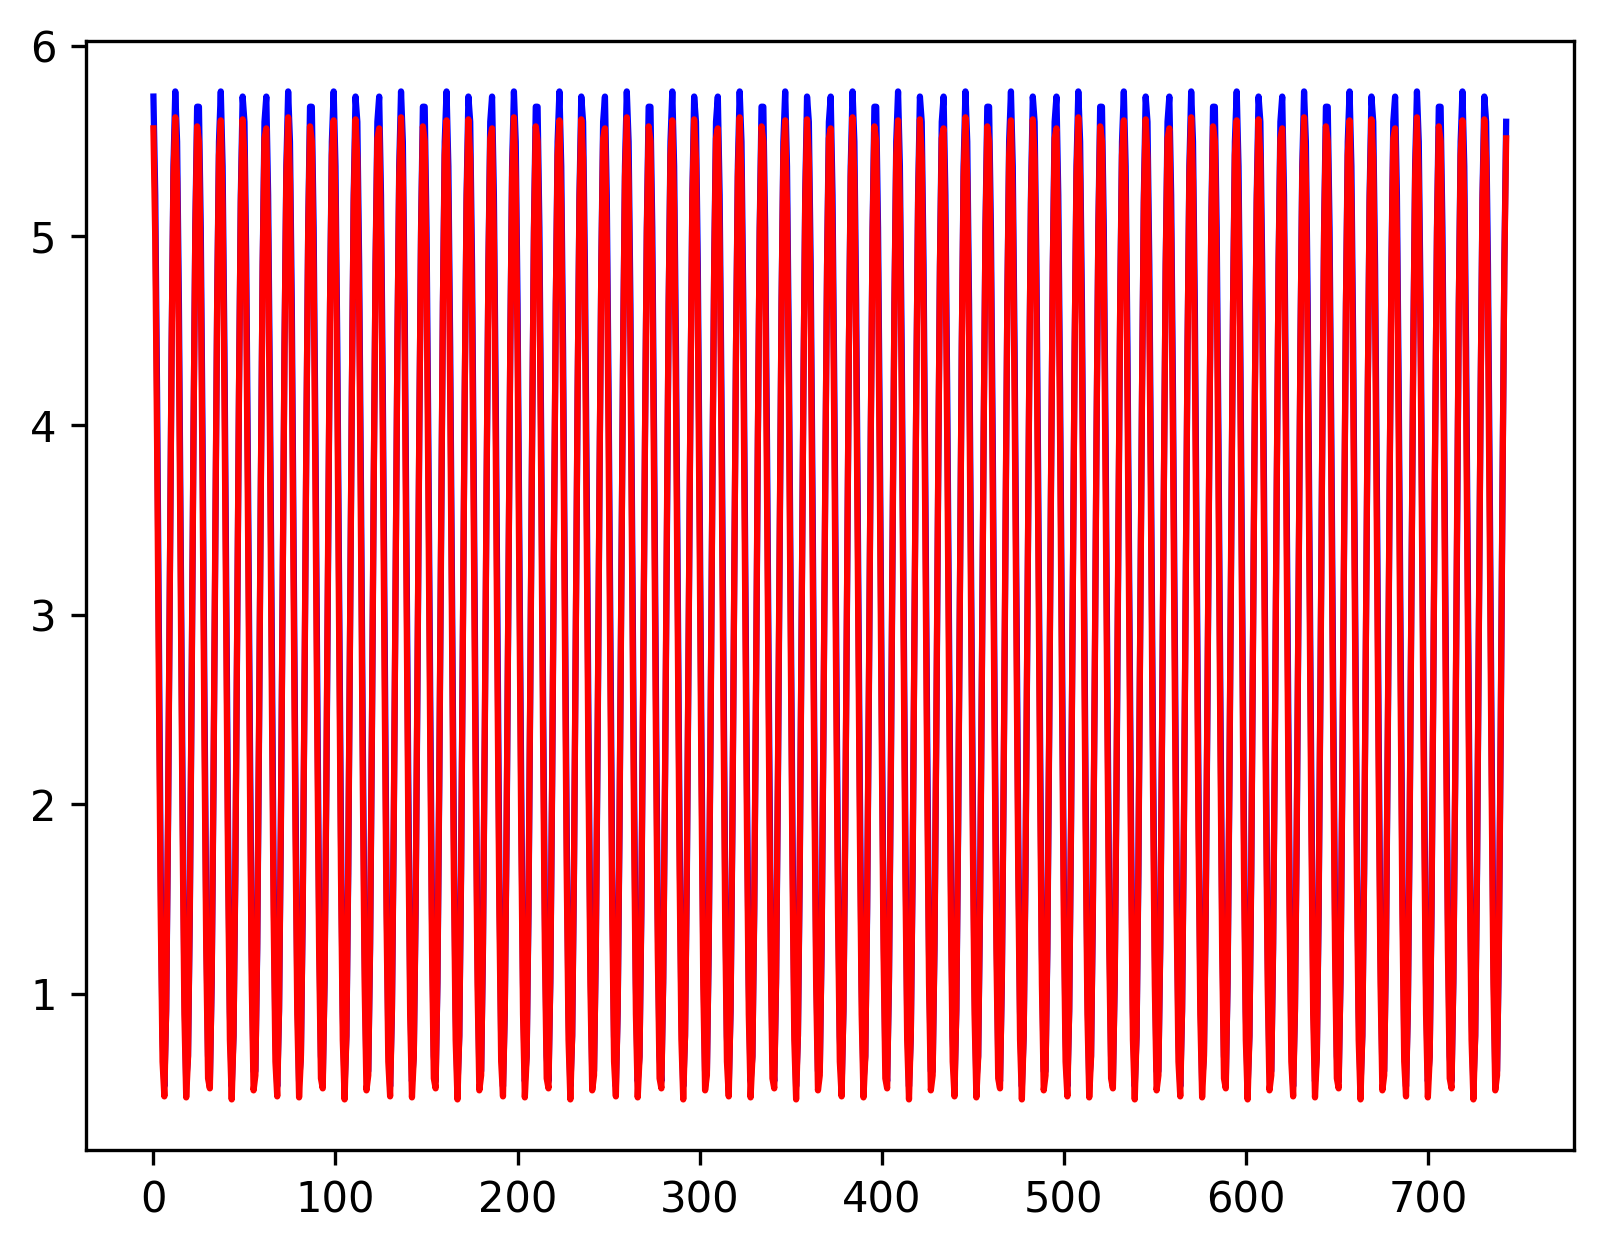
\includegraphics[scale=1]{ Images/aprox_enero_aprox_marzo.png}\\
     \captionof{figure}{Resultado de los cálculos de las series, usando distintos subsets de datos: Enero y Marzo.}
     \label{fig:fig2}
\end{minipage}
   
Para calcular las pleamares fue necesario estimar la frecuencia angular del primer armónico $\omega_1$, para ello hallamos la diferencia promedio de tiempo en minutos entre las pleamares y luego las promediamos. 
Por último resolvimos el sistema \ref{eq_15} y hallamos los siguientes valores.

\begin{verbatim}
    El valor estimado para la frecuencia w_1:  0.008462076602440048
    Coeficientes para calcular el modelo:  [ 1.00839372  0.1493136  -0.50259993]
    Error Cuadrático Medio del Modelo:  0.47478065159866845    
\end{verbatim}

Por último, utilizamos los resultados para modelar las marealtas y hallamos la primer marea alta de junio, ingresando los minutos correspondientes a la funcion $altura_1(t)$, resultando que el primer máximo está a las (00:01) del primero de junio.


\section{\underline{Conclusiones}}

En el análisis de los resultados, de las estimaciones de errores cuadraticos medios, y en el espectro de la distribución de mareas, podemos inferir que la ley que rige a las mareas no corresponde a una suma de senos y cosenos, como la literatura cuenta que utilizó Fourier para inspirarse y desarrollar su serie, sin embargo tomando los modelos que podemos conseguir aun nos pueden dar información útil, como predecir las mareas.

\section{\underline{Anexo I}}



\subsection{Funciones}
\begin{verbatim}
import numpy as np
import os
import pandas as pd
from matplotlib import pyplot as plt
from datetime import datetime

root_file = os.path.dirname(os.path.realpath(__file__))

#Esta funcion obtiene como entrada dos fechas en formato "AAAA/MM/DD HH:mm". En caso de invocarse vacía devuelve todo el set.
def leer_archivo_maine(fecha_inicio = "",fecha_fin = ""):
    #Defino un Formato de Fecha
    format = "%Y/%m/%d %H:%M"
    #Cargo un objeto del tipo Panda, con el resultado del archivo
    alturas_mareas = pd.read_csv('CO-OPS_8410140_met-2019.csv', 
        parse_dates = {'DateTime': [0,1]},
        date_parser = lambda x: datetime.strptime(x,format)
    )
    #Pregunto si hay parámetros de entrada.
    if( fecha_inicio == "" or fecha_fin == ""):
        return alturas_mareas
    else:
        #Seteo una mascara con condicion de verdad para los resultados que busco
        mask = ((alturas_mareas["DateTime"] <= datetime.strptime(fecha_fin,format)) & (alturas_mareas["DateTime"] >= datetime.strptime(fecha_inicio,format)))
        return alturas_mareas.loc[mask]

def procesar_archivo_mar_del_plata():
    #leo el archivo
    alturas_mareas = pd.read_csv(root_file+"/Mar-del-plata.csv")
    fechas = alturas_mareas['fecha_hora']
    alturas = alturas_mareas['altura']
    valor_medio_marea = np.mean(alturas)
    format = "%d/%m/%y %H:%M:%S"
    diffs = []
    minutes = []
    pleamares = []
    for index, f in enumerate(fechas):
        es_pleamar = alturas[index] > valor_medio_marea
        pleamares.append(es_pleamar)
        if (index == 0):
            diffs.append(0.0)
            minutes.append(0.0)
        else:
            d0 = datetime.strptime(fechas[index - 1], format)
            d1 = datetime.strptime(f, format)
            secs = (d1 - d0).total_seconds()/60
            next_val = secs + minutes[index - 1]
            minutes.append(int(next_val))
            diffs.append(int(secs))

    alturas_mareas["t_minutos"] = minutes
    alturas_mareas["i_minutos"] = diffs
    alturas_mareas["es_pleamar"] = pleamares

    alturas_mareas.to_csv(root_file+"/Mar-Del-Plata-Normalizado.csv")

def leer_archivo_mar_del_plata_normalizado():
    return pd.read_csv(root_file+"/Mar-Del-Plata-Normalizado.csv")

def fft_datos(datos):
    #Obtengo el numero de datos
    N = len(datos)
    #Normalizo los Datos, dividiendolos por la cantidad de muestras útiles
    datos_fft = np.fft.fft(datos)[:int(N/2)]*2/N
    #Debido al shifting, el armónico 0 se duplica, dado que el espectro se repite a partir de la posicion N+1, que se vuelve a copiar en la posicion 0
    datos_fft[0] = datos_fft[0]/2
    return datos_fft
    


#Defino el coeficiente A_k según lo calculado
def A_k(a_k, f_k):
    return a_k * np.cos(f_k)
#Defino el coeficiente B_k según lo calculado
def B_k(b_k, f_k):
    return -b_k * np.sin(f_k)

#Utilizo la serie de fourier para reconstruir la señal
#datos_fft son todos los coeficientes de fourier complejos
#ind corresponde a los indices de los armónicos deseados
#t corresponde al array de tiempo. Este debe estar en la misma unidad que el tiempo de las muestras a partir se calculo la fft.
def sf_altura(datos_fft,t,ind = []):

    w_0 = 2*np.pi/(2*len(datos_fft))
    acc = 0
    #si no tengo armonicos elegidos, itero sobre todos los datos
    if(len(ind)==0):
        ind = np.arange(len(datos_fft))
    #itero sobre los armonicos seleccionados
    for k in ind:
        amp = np.abs(datos_fft[k])
        ang = np.angle(datos_fft[k])
        a_k = A_k(amp,ang)
        b_k = B_k(amp,ang)
        acc = (a_k * np.cos(w_0 * k * t)) + (b_k * np.sin(w_0 * k * t)) + acc
    return acc

#Esta funcion obtiene los indices de los armónicos mas altos
def obtener_indices_armonicos(datos_fft,n_armonicos):
    #Primero Ordeno los elementos de menor a mayor
    #Luego invierto el array para que quede de mayor a menor
    #Por ultimo tomo los n_armonicos mas altos
    maximos = np.flip(np.sort(datos_fft))[0:n_armonicos]
    #Luego filtro a los elementos menores al menor de los maximos, los vuelvo 0
    datos_fft_mayores_a_maximos = np.where(
        datos_fft < np.min(maximos),
        0,
        datos_fft)
    #Regreso los elementos 
    return np.nonzero(datos_fft_mayores_a_maximos)[0]

#implemento la definicion del Error Cuadratico Medio
def ECM(A,B):
    return np.sqrt(np.mean((A - B)**2))

#Esta funcion tabula el error cuadrático medio, segun la cantidad de armónicos utilizados para calcular la serie de fourier
def obtener_error_cuadratico_segun_numero_muestras(n,mediciones,mediciones_fft,filename=""):
    data = []
    media_ = np.mean(mediciones)
    for i in np.arange(n):
        numero_armonico = i+1
        indices_n = obtener_indices_armonicos(mediciones_fft,numero_armonico)
        serie_fourier_alturas_h = sf_altura(mediciones_fft,np.arange(len(mediciones)),indices_n)
        ecm = ECM(mediciones,serie_fourier_alturas_h)
        #print(numero_armonico, ecm, (ecm/media_ * 100))
        data.append([numero_armonico,ecm,(ecm/media_ * 100)])
    ec_panda = pd.DataFrame(data,columns=["Numero de Armónico","E.C.M.","ECM%"])
    if(filename != ""):
        ec_panda.to_csv(filename)
    return ec_panda


#en el informe se muestra como llegamos a estas ecuaciones
def calcular_coeficientes_c_i(minutes,alturas,w_1):
    Q11 = sum(1 for i,y in enumerate(alturas) )
    Q22 = sum(np.cos(w_1*minutes[i])**2 for i, x in enumerate(alturas))
    Q33 = sum(np.sin(w_1*minutes[i])**2 for i, x in enumerate(alturas))
    Q12 = sum(np.cos(w_1*minutes[i]) for i, x in enumerate(alturas))
    Q23 = sum(np.sin(w_1*minutes[i]) for i, x in enumerate(alturas))
    Q13 = sum(np.cos(w_1*minutes[i])*np.sin(w_1*minutes[i]) for i, x in enumerate(alturas))

    Y1 = sum(y for i, y in enumerate(alturas))
    Y2 = sum(y*np.cos(w_1*minutes[i]) for i, y in enumerate(alturas))
    Y3 = sum(y*np.sin(w_1*minutes[i]) for i, y in enumerate(alturas))

    
    a = np.matrix([[Q11, Q12, Q13],[Q12,Q22,Q23],[Q13,Q23,Q33]])
    b = np.array([Y1, Y2, Y3])
    c = np.linalg.solve(a, b)
    return c


#Esta funcion representa a la funcion alturas para el primer armónico.
#params[0] = a_0
#params[1] = a_1
#params[2] = w_1
#params[3] = phi_1
def alturas_1(params,t):
    return params[0] + params[1]*np.cos(params[2]*t+params[3])

def alturas_1_f(params,w_1,t):
    return params[0] + params[1]*np.cos(w_1*t)- params[2]*np.sin(w_1*t)
    
def alturas_1_g(t):
    print(t)
    params = [ 1.00839372 , 0.1493136 , -0.50259993]
    w_1 = 0.008462076602440048
    return params[0] + params[1]*np.cos(w_1*t)- params[2]*np.sin(w_1*t)

def plot_log(name,x,y,x_label,y_label,show = False):
    plt.plot(x,y,'b-')
    plt.yscale("log")
    plt.xlabel = x_label
    plt.ylabel = y_label
    plt.savefig( root_file+'/Images/'+name+'.png', dpi=300, bbox_inches='tight')
    if(show):
        plt.show()
    
def plot(name,x,y,x_label,y_label,show = False):
    plt.plot(x,y,'b-')
    plt.xlabel = x_label
    plt.ylabel = y_label
    plt.yscale("linear")
    plt.savefig( root_file+'/Images/'+name+'.png', dpi=300, bbox_inches='tight')
    if(show):
        plt.show()

\end{verbatim}

\subsection{Ejercicio A}

\begin{verbatim}
import funciones as f
import numpy as np
import pandas as pd


#El objetivo de este este ejercicio es seleccionar los armónicos que aportan información.

mediciones_alturas = f.leer_archivo_maine()['Verified (m)']
N_samples = int(len(mediciones_alturas))
tiempo = np.arange(N_samples)
mediciones_alturas_fft = f.fft_datos(mediciones_alturas)
W_samples = int(len(mediciones_alturas_fft))
omega = np.arange(W_samples) * (2*np.pi/N_samples)
freq = np.arange(W_samples) / N_samples
serie_fourier_alturas = f.sf_altura(mediciones_alturas_fft,tiempo)

#graficamos los armonicos

f.plot_log("ejercicio_a_fft_log",freq,np.abs(mediciones_alturas_fft),"Frecuencia [1/H]","Amplitud [m]")

#Comparamos el error cuadrático medio segun la cantidad de maximos de la fft que tomamos:
numero_de_armonicos = 12
pd_ecm_x_n = f.obtener_error_cuadratico_segun_numero_muestras(numero_de_armonicos,mediciones_alturas,mediciones_alturas_fft,'ecm_por_'+str(numero_de_armonicos)+'_armonicos.csv')

f.plot("ejercicio_a_ecm_x_"+str(numero_de_armonicos)+"armonicos",np.arange(len(pd_ecm_x_n["ECM%"])),pd_ecm_x_n["ECM%"],"Numero de Armonicos","Error Cuadratico Medio Porcentual")

#Se decide que con los primeros 3 armonicos se comete un error del 30%, y para bajarlo a menos de 25 se necesitan mas de 10 armónicos. 
print(Errorpd_ecm_x_n)
\end{verbatim}
\subsection{Ejercicio B}
\begin{verbatim}
    import funciones as f
import numpy as np
import pandas as pd


#El objetivo de este este ejercicio es obtener una descomposición armónica mediante la FFT, 
#y obtener los coeficientes de fourier a partir de las N armónicos elegidos del ejercicio anterior
N_armonicos = 4
mediciones_alturas = f.leer_archivo_maine()['Verified (m)']
N_samples = int(len(mediciones_alturas))
tiempo = np.arange(N_samples)
mediciones_alturas_fft = f.fft_datos(mediciones_alturas)
W_samples = int(len(mediciones_alturas_fft))
omega = np.arange(W_samples) * (2*np.pi/N_samples)
freq = np.arange(W_samples) / N_samples
indices_armonicos = f.obtener_indices_armonicos(mediciones_alturas_fft,N_armonicos)
serie_fourier_alturas = f.sf_altura(mediciones_alturas_fft,tiempo,indices_armonicos)

ecm_n = f.ECM(serie_fourier_alturas,mediciones_alturas)

print("El E.C.M para "+str(N_armonicos)+" armónicos es: ",ecm_n)
print("Las Frecuencias Usadas son: ", indices_armonicos/N_samples)

\end{verbatim}
\subsection{Ejercicio C}
\begin{verbatim}
    import funciones as f
import numpy as np
import pandas as pd


#El objetivo de este este ejercicio es obtener una descomposición armónica mediante la FFT, 
#y obtener los coeficientes de fourier a partir de las N armónicos elegidos del ejercicio anterior
N_armonicos = 3
mediciones_alturas = f.leer_archivo_maine()['Verified (m)']
N_samples = int(len(mediciones_alturas))
tiempo = np.arange(N_samples)
mediciones_alturas_fft = f.fft_datos(mediciones_alturas)
W_samples = int(len(mediciones_alturas_fft))
omega = np.arange(W_samples) * (2*np.pi/N_samples)
freq = np.arange(W_samples) / N_samples
indices_armonicos = f.obtener_indices_armonicos(mediciones_alturas_fft,N_armonicos)
serie_fourier_alturas = f.sf_altura(mediciones_alturas_fft,tiempo,indices_armonicos)

ecm_n = f.ECM(serie_fourier_alturas,mediciones_alturas)

print("El E.C.M para "+str(N_armonicos)+" armónicos es: ",ecm_n)
print("Las Frecuencias Usadas son: ", indices_armonicos/N_samples)
\end{verbatim}
\subsection{Ejercicio D}
\begin{verbatim}
    import funciones as f
import numpy as np
import pandas as pd
import datetime as dt

#El objetivo de este ejercicio es analizar sub muestras y procesarlas según un rango de fecha.
#El formato de las fechas es 
format = "%Y/%m/%d %H:%M"
fechas = [
    {"Descripcion":"Primer Semana de Enero" ,"sFechaInicio":"2019/01/01 00:00","sFechaFin":"2019/01/07 23:00"},
    {"Descripcion":"Segunda Semana de Enero" ,"sFechaInicio":"2019/01/08 00:00","sFechaFin":"2019/01/14 23:00"},
    {"Descripcion":"Enero y Febrero" ,"sFechaInicio":"2019/01/01 00:00","sFechaFin":"2019/03/01 00:00"},
    {"Descripcion":"Marzo y Abril" ,"sFechaInicio":"2019/01/01 00:00","sFechaFin":"2019/03/01 00:00"},
]



N_armonicos = 4
for fecha in fechas:
    print(fecha)
    mediciones_alturas = f.leer_archivo_maine(fecha["sFechaInicio"],fecha["sFechaFin"])['Verified (m)']
    N_samples = int(len(mediciones_alturas))
    tiempo = np.arange(N_samples)
    mediciones_alturas_fft = f.fft_datos(mediciones_alturas)
    W_samples = int(len(mediciones_alturas_fft))
    omega = np.arange(W_samples) * (2*np.pi/N_samples)
    freq = np.arange(W_samples) / N_samples
    #Calculo para los  4 armónicos principales
    indices_armonicos = f.obtener_indices_armonicos(mediciones_alturas_fft,N_armonicos)
    serie_fourier_alturas = f.sf_altura(mediciones_alturas_fft,tiempo,indices_armonicos)
    ecm_n = f.ECM(serie_fourier_alturas,mediciones_alturas)
    print("Las frecuencias utilizadas son :",freq[indices_armonicos])
    print("El E.C.M para el rango de fechas de "+fecha["sFechaInicio"]+" hasta "+fecha["sFechaFin"]+" con "+str(N_armonicos)+" armónicos es: ",ecm_n)
    #Calculo para los 3 armónicos principales
    indices_armonicos = f.obtener_indices_armonicos(mediciones_alturas_fft,N_armonicos-1)
    serie_fourier_alturas = f.sf_altura(mediciones_alturas_fft,tiempo,indices_armonicos)
    ecm_n = f.ECM(serie_fourier_alturas,mediciones_alturas)
    print("El E.C.M para el rango de fechas de "+fecha["sFechaInicio"]+" hasta "+fecha["sFechaFin"]+" con "+str(N_armonicos-1)+" armónicos es: ",ecm_n)
    



\end{verbatim}
\subsection{Ejercicio E}
\begin{verbatim}
    from numpy.core.numeric import indices
import funciones as f
import numpy as np
import pandas as pd
import datetime as dt
from matplotlib import pyplot as plt


#Debemos aplicar este modelo a nuestros datos

#altura = a_0 + a_1 * cos(w_1 *t + phi_1)

#Sabemos que el valor a_0 es el valor medio
N_armonicos = 2 
mediciones_alturas_enero = f.leer_archivo_maine("2019/01/01 00:00","2019/01/31 23:00")['Verified (m)']
mediciones_alturas_marzo = f.leer_archivo_maine("2019/03/01 00:00","2019/03/31 23:00")['Verified (m)']

n_alturas_enero = len(mediciones_alturas_enero)
n_alturas_marzo = len(mediciones_alturas_marzo)

t_enero = np.arange(n_alturas_enero)
t_marzo = np.arange(n_alturas_marzo)

fft_enero = f.fft_datos(mediciones_alturas_enero)
fft_marzo = f.fft_datos(mediciones_alturas_marzo)

indices_armonicos_enero = f.obtener_indices_armonicos(fft_enero,N_armonicos)
indices_armonicos_marzo = f.obtener_indices_armonicos(fft_marzo,N_armonicos)

n_fft_enero = len(fft_enero)
n_fft_marzo = len(fft_marzo)

#ordeno los parámetros en un array [a_0,a_1,w_1,phi_1]
print("Indices Armonicos Enero",indices_armonicos_enero)
print("Indices Armonicos Marzo",indices_armonicos_marzo)

parametros_enero = [np.abs(fft_enero[0]),np.abs(fft_enero[indices_armonicos_enero[1]]), indices_armonicos_enero[1] * (2*np.pi/n_alturas_enero),np.angle(fft_enero[indices_armonicos_enero[1]])]
parametros_marzo = [np.abs(fft_marzo[0]),np.abs(fft_marzo[indices_armonicos_marzo[1]]), indices_armonicos_marzo[1] * (2*np.pi/n_alturas_marzo),np.angle(fft_marzo[indices_armonicos_marzo[1]])] 

print("Valor Medio Enero (a_0): ",parametros_enero[0],", Primer Armónico (a_1): ",parametros_enero[1]," Frecuencia Angular (w_1): ",parametros_enero[2], " Fase 1 (phi_1): ",parametros_enero[3])
print("Valor Medio marzo (a_0): ",parametros_marzo[0],", Primer Armónico (a_1): ",parametros_marzo[1]," Frecuencia Angular (w_1): ",parametros_marzo[2], " Fase 1 (phi_1): ",parametros_marzo[3])

sf_enero = f.sf_altura(fft_enero,np.arange(n_alturas_enero),indices_armonicos_enero)
sf_marzo = f.sf_altura(fft_marzo,np.arange(n_alturas_marzo),indices_armonicos_marzo)

aprox_enero = f.alturas_1(parametros_enero,t_enero)
aprox_marzo = f.alturas_1(parametros_marzo,t_marzo)

print("diff SF vs aprox Enero", f.ECM(aprox_enero,sf_enero),f.ECM(aprox_enero,mediciones_alturas_enero))
print("diff SF vs aprox Marzo", f.ECM(aprox_marzo,sf_marzo),f.ECM(aprox_marzo,mediciones_alturas_marzo))

ECM_enero = f.ECM(sf_enero,mediciones_alturas_enero)
ECM_marzo = f.ECM(sf_marzo,mediciones_alturas_marzo)

print("ECM Enero",ECM_enero)
print("ECM Marzo",ECM_marzo)

ECM_enero_marzo = f.ECM(sf_enero,mediciones_alturas_marzo)
ECM_marzo_enero = f.ECM(sf_marzo,mediciones_alturas_enero)

print("ECM Enero predicho con Marzo",ECM_enero)
print("ECM Marzo predicho con Enero",ECM_marzo)


"""
plt.plot(np.arange(n_fft_enero),np.abs(fft_enero),'b-',np.arange(n_fft_marzo),np.abs(fft_marzo),'r')
plt.yscale("log")
plt.show()
"""
plt.plot(t_enero,aprox_enero,'b',t_marzo,aprox_marzo,'r')
plt.yscale("linear")
plt.savefig(f.root_file+'/Images/aprox_enero_aprox_marzo.png', dpi=300, bbox_inches='tight')






\end{verbatim}
\subsection{Ejercicio F}
\begin{verbatim}
    from numpy.core.defchararray import index
from numpy.core.numeric import indices
import funciones as f
import numpy as np
import pandas as pd
import datetime as dt
from matplotlib import pyplot as plt

#En este ejercicio, las muestras del archivo Mar-del-plata.csv no son equiespaciadas y registran solo pleamares y bajamares. Y los registros estan en minutos. 
#La menor unidad de tiempo que usaremos será el minuto
#Primero procesamos el archivo y obtenemos una versión que ademas de tener las columnas de fecha y altura, se le agregan las columnas que guarden:
#t_minutos: los minutos desde la primer muestra
#i_minutos: los munutos desde la muestra anterior
#es_pleamar: si es pleamar o bajamar

f.procesar_archivo_mar_del_plata()
alturas = f.leer_archivo_mar_del_plata_normalizado()

#luego podemos obtener, nuestro pares {x,y}

#nuevamente queremos utilizar la funcion a_0 + a_1 cos(w_1 *t + phi_1) para aproximar estos datos.
#esta funcion se puede reescribir como  a_0 * 1 + a_1 * cos(w_1 *t ) + b_1 * sen (w_1 * t)
#en este caso, el conjunto de phi_i(x) = {1,cos(w_1*t),sen(w_1*t)} y queremos saber los c_i {a_0,a_1,b_1}
#asumimos que w_1 es correspondiente a 2pi/Tpleamares, tambien podemos usar como dato que la pleamar ocurre cada 12 horas, entonces w_1 = 2pi / (12*60)

X = alturas['t_minutos']
Y = alturas['altura']

T_pleamar = sum(alturas["i_minutos"])/ (0.5*len(alturas["i_minutos"]))

w_1 = 2*np.pi / T_pleamar

print("El valor estimado para la frecuencia w_1: ",w_1)

c_i = f.calcular_coeficientes_c_i(X,Y,w_1)

print("Coeficientes para calcular el modelo: ",c_i)
modelo = f.alturas_1_f(c_i,w_1,Y)
ECM_modelo = f.ECM(Y,modelo)

print("Error Cuadrático Medio del Modelo: ",ECM_modelo)

#print(alturas)

\end{verbatim}
\subsection{Ejercicio G}
\begin{verbatim}
    
from numpy.core.defchararray import index
from numpy.core.numeric import indices
import funciones as f
import numpy as np
import pandas as pd
import datetime as dt
from matplotlib import pyplot as plt

alturas = f.leer_archivo_mar_del_plata_normalizado()

minutes= alturas["t_minutos"]
#Del 21/05/2021 el ultimo dato es a las 19:49. 
#hay 11 minutos hasta las 20
#hay 251 minutos hasta las 00:00 del 22.
#hay 10 dias del 22 al primero de junio 10*24*60 +251 = 

t_inicial = (int)(minutes[len(minutes)-1] + 251+ 10*24*60)
#10 horas
t_final = t_inicial + 60

t_junio = np.arange(t_inicial,t_final,1)

calculado_junio = f.alturas_1_g(t_junio)

t_junio_maximos = np.argmax(calculado_junio)



print("El primer máximo es a los ",t_junio_maximos+1,"minutos del primero de junio")

\end{verbatim}


\section{\underline{Anexo II}}
\subsection{Ejercicio A}
\begin{verbatim}
    Numero de Armónico    E.C.M.       ECM%
    0                    1  1.976309  64.276293
    1                    2  1.932768  62.860197
    2                    3  0.982349  31.949333
    3                    4  0.979766  31.865318
    4                    5  0.975433  31.724401
    5                    6  0.973297  31.654926
    6                    7  0.911776  29.654046
    7                    8  0.888934  28.911155
    8                    9  0.878138  28.560047
    9                   10  0.874409  28.438738
    10                  11  0.867637  28.218507
    11                  12  0.865495  28.148833
\end{verbatim}
\subsection{Ejercicio B}
\begin{verbatim}
    El E.C.M para 4 armónicos es:  0.9797659067456904
    Las Frecuencias Usadas son:  [0.         0.03869863 0.07899543 0.08047945]
\end{verbatim}
\subsection{Ejercicio C}
\begin{verbatim}
    El E.C.M para 3 armónicos es:  0.9823491454457174
    Las Frecuencias Usadas son:  [0.         0.07899543 0.08047945]
\end{verbatim}
\subsection{Ejercicio D}
\begin{verbatim}
    {'Descripcion': 'Primer Semana de Enero', 'sFechaInicio': '2019/01/01 00:00', 'sFechaFin': '2019/01/07 23:00'}
Las frecuencias utilizadas son : [0.         0.08333333 0.08928571 0.0952381 ]
El E.C.M para el rango de fechas de 2019/01/01 00:00 hasta 2019/01/07 23:00 con 4 armónicos es:  1.2367958297155777
El E.C.M para el rango de fechas de 2019/01/01 00:00 hasta 2019/01/07 23:00 con 3 armónicos es:  1.2659584466847664
{'Descripcion': 'Segunda Semana de Enero', 'sFechaInicio': '2019/01/08 00:00', 'sFechaFin': '2019/01/14 23:00'}
Las frecuencias utilizadas son : [0.         0.06547619 0.07142857 0.07738095]
El E.C.M para el rango de fechas de 2019/01/08 00:00 hasta 2019/01/14 23:00 con 4 armónicos es:  1.4869772458332933
El E.C.M para el rango de fechas de 2019/01/08 00:00 hasta 2019/01/14 23:00 con 3 armónicos es:  1.500698778195625
{'Descripcion': 'Enero y Febrero', 'sFechaInicio': '2019/01/01 00:00', 'sFechaFin': '2019/03/01 00:00'}
Las frecuencias utilizadas son : [0.         0.07904023 0.07974594 0.08045166]
El E.C.M para el rango de fechas de 2019/01/01 00:00 hasta 2019/03/01 00:00 con 4 armónicos es:  0.6826298627212011
El E.C.M para el rango de fechas de 2019/01/01 00:00 hasta 2019/03/01 00:00 con 3 armónicos es:  0.6696914537749843
{'Descripcion': 'Marzo y Abril', 'sFechaInicio': '2019/01/01 00:00', 'sFechaFin': '2019/03/01 00:00'}
Las frecuencias utilizadas son : [0.         0.07904023 0.07974594 0.08045166]
El E.C.M para el rango de fechas de 2019/01/01 00:00 hasta 2019/03/01 00:00 con 4 armónicos es:  0.6826298627212011
El E.C.M para el rango de fechas de 2019/01/01 00:00 hasta 2019/03/01 00:00 con 3 armónicos es:  0.6696914537749843
\end{verbatim}
\subsection{Ejercicio E}
\begin{verbatim}
    Indices Armonicos Enero [ 0 60]
Indices Armonicos Marzo [ 0 60]
Valor Medio Enero (a_0):  3.1356599462365593 , Primer Armónico (a_1):  2.6293397521253157  Frecuencia Angular (w_1):  0.5067084925144828  Fase 1 (phi_1):  0.1522951793391947
Valor Medio marzo (a_0):  3.033045698924731 , Primer Armónico (a_1):  2.5921290112734927  Frecuencia Angular (w_1):  0.5067084925144828  Fase 1 (phi_1):  0.21275576895293635
diff SF vs aprox Enero 1.6433518802278473e-14 0.648268327126505
diff SF vs aprox Marzo 1.4118211352582575e-14 0.7298623680117619
ECM Enero 0.6482683271265038
ECM Marzo 0.7298623680117596
ECM Enero predicho con Marzo 0.6482683271265038
ECM Marzo predicho con Enero 0.7298623680117596
\end{verbatim}
\subsection{Ejercicio F}
\begin{verbatim}
    El valor estimado para la frecuencia w_1:  0.008462076602440048
Coeficientes para calcular el modelo:  [ 1.00839372  0.1493136  -0.50259993]
Error Cuadrático Medio del Modelo:  0.47478065159866845
\end{verbatim}
\subsection{Ejercicio G}
\begin{verbatim}
    132339 132340 132341 132342 132343 132344 132345 132346 132347 132348
 132349 132350 132351 132352 132353 132354 132355 132356 132357 132358
 132359 132360 132361 132362 132363 132364 132365 132366 132367 132368
 132369 132370 132371 132372 132373 132374 132375 132376 132377 132378
 132379 132380 132381 132382 132383 132384 132385 132386 132387 132388
 132389 132390 132391 132392 132393 132394 132395 132396 132397 132398]
El primer máximo es a los  1 minutos del primero de junio
\end{verbatim}

%%%%%%%%%%%%%%%%%%%%%%%%%%%%%%%%%%%%%%%%%%%%%%%%%%%%%%%%%%%%%%%%%%%%%%%%%%%%%%%%%%%%%%%%%%%%%%%%%%%%%%%%%%%%%%
\section{\underline{Bibliografía}}
\begin{thebibliography}{9}

\bibitem{ana1} 
Hernán González (2017) - Análisis Numérico Primer Curso 2º ediciòn. Buenos Aires. Nueva Librería. 
\bibitem{ana2}
Burden, Richard L. / J. Douglas Faires (2011) - Análisis Numérico, Novena edición. Cengage Learning.
\bibitem{sys}
Oppenheim Alan V. / Willsky Allan S. (1997) - Signals And Systems, Second Edition. Prentice Hall.
\end{thebibliography}




\end{document}
